\documentclass[final,hyperref={pdfpagelabels=false}]{beamer}

\usepackage[
    size=custom,
    orientation=landscape,
    width=121.92,  % 4'
    height=76.2,  % 30''
    scale=1.45,
]{beamerposter}
\usetheme{I6pd2}

\usepackage[utf8x]{inputenc}
\usepackage[T1]{fontenc}
\usepackage{lmodern}
\usepackage{enumerate}
\usepackage{graphicx}
\usepackage{hyperref}
\usepackage{booktabs}
\usepackage{fancyvrb}
\usepackage{color}

\usecaptiontemplate{\small\structure{\insertcaptionname~\insertcaptionnumber: }\insertcaption}
\addtobeamertemplate{block end}{}{\vspace*{2ex}}

% Coconut highlighting
\makeatletter
\def\PY@reset{\let\PY@it=\relax \let\PY@bf=\relax%
    \let\PY@ul=\relax \let\PY@tc=\relax%
    \let\PY@bc=\relax \let\PY@ff=\relax}
\def\PY@tok#1{\csname PY@tok@#1\endcsname}
\def\PY@toks#1+{\ifx\relax#1\empty\else%
    \PY@tok{#1}\expandafter\PY@toks\fi}
\def\PY@do#1{\PY@bc{\PY@tc{\PY@ul{%
    \PY@it{\PY@bf{\PY@ff{#1}}}}}}}
\def\PY#1#2{\PY@reset\PY@toks#1+\relax+\PY@do{#2}}

\expandafter\def\csname PY@tok@w\endcsname{\def\PY@tc##1{\textcolor[rgb]{0.73,0.73,0.73}{##1}}}
\expandafter\def\csname PY@tok@c\endcsname{\let\PY@it=\textit\def\PY@tc##1{\textcolor[rgb]{0.25,0.50,0.50}{##1}}}
\expandafter\def\csname PY@tok@cp\endcsname{\def\PY@tc##1{\textcolor[rgb]{0.74,0.48,0.00}{##1}}}
\expandafter\def\csname PY@tok@k\endcsname{\let\PY@bf=\textbf\def\PY@tc##1{\textcolor[rgb]{0.00,0.50,0.00}{##1}}}
\expandafter\def\csname PY@tok@kp\endcsname{\def\PY@tc##1{\textcolor[rgb]{0.00,0.50,0.00}{##1}}}
\expandafter\def\csname PY@tok@kt\endcsname{\def\PY@tc##1{\textcolor[rgb]{0.69,0.00,0.25}{##1}}}
\expandafter\def\csname PY@tok@o\endcsname{\def\PY@tc##1{\textcolor[rgb]{0.40,0.40,0.40}{##1}}}
\expandafter\def\csname PY@tok@ow\endcsname{\let\PY@bf=\textbf\def\PY@tc##1{\textcolor[rgb]{0.67,0.13,1.00}{##1}}}
\expandafter\def\csname PY@tok@nb\endcsname{\def\PY@tc##1{\textcolor[rgb]{0.00,0.50,0.00}{##1}}}
\expandafter\def\csname PY@tok@nf\endcsname{\def\PY@tc##1{\textcolor[rgb]{0.00,0.00,1.00}{##1}}}
\expandafter\def\csname PY@tok@nc\endcsname{\let\PY@bf=\textbf\def\PY@tc##1{\textcolor[rgb]{0.00,0.00,1.00}{##1}}}
\expandafter\def\csname PY@tok@nn\endcsname{\let\PY@bf=\textbf\def\PY@tc##1{\textcolor[rgb]{0.00,0.00,1.00}{##1}}}
\expandafter\def\csname PY@tok@ne\endcsname{\let\PY@bf=\textbf\def\PY@tc##1{\textcolor[rgb]{0.82,0.25,0.23}{##1}}}
\expandafter\def\csname PY@tok@nv\endcsname{\def\PY@tc##1{\textcolor[rgb]{0.10,0.09,0.49}{##1}}}
\expandafter\def\csname PY@tok@no\endcsname{\def\PY@tc##1{\textcolor[rgb]{0.53,0.00,0.00}{##1}}}
\expandafter\def\csname PY@tok@nl\endcsname{\def\PY@tc##1{\textcolor[rgb]{0.63,0.63,0.00}{##1}}}
\expandafter\def\csname PY@tok@ni\endcsname{\let\PY@bf=\textbf\def\PY@tc##1{\textcolor[rgb]{0.60,0.60,0.60}{##1}}}
\expandafter\def\csname PY@tok@na\endcsname{\def\PY@tc##1{\textcolor[rgb]{0.49,0.56,0.16}{##1}}}
\expandafter\def\csname PY@tok@nt\endcsname{\let\PY@bf=\textbf\def\PY@tc##1{\textcolor[rgb]{0.00,0.50,0.00}{##1}}}
\expandafter\def\csname PY@tok@nd\endcsname{\def\PY@tc##1{\textcolor[rgb]{0.67,0.13,1.00}{##1}}}
\expandafter\def\csname PY@tok@s\endcsname{\def\PY@tc##1{\textcolor[rgb]{0.73,0.13,0.13}{##1}}}
\expandafter\def\csname PY@tok@sd\endcsname{\let\PY@it=\textit\def\PY@tc##1{\textcolor[rgb]{0.73,0.13,0.13}{##1}}}
\expandafter\def\csname PY@tok@si\endcsname{\let\PY@bf=\textbf\def\PY@tc##1{\textcolor[rgb]{0.73,0.40,0.53}{##1}}}
\expandafter\def\csname PY@tok@se\endcsname{\let\PY@bf=\textbf\def\PY@tc##1{\textcolor[rgb]{0.73,0.40,0.13}{##1}}}
\expandafter\def\csname PY@tok@sr\endcsname{\def\PY@tc##1{\textcolor[rgb]{0.73,0.40,0.53}{##1}}}
\expandafter\def\csname PY@tok@ss\endcsname{\def\PY@tc##1{\textcolor[rgb]{0.10,0.09,0.49}{##1}}}
\expandafter\def\csname PY@tok@sx\endcsname{\def\PY@tc##1{\textcolor[rgb]{0.00,0.50,0.00}{##1}}}
\expandafter\def\csname PY@tok@m\endcsname{\def\PY@tc##1{\textcolor[rgb]{0.40,0.40,0.40}{##1}}}
\expandafter\def\csname PY@tok@gh\endcsname{\let\PY@bf=\textbf\def\PY@tc##1{\textcolor[rgb]{0.00,0.00,0.50}{##1}}}
\expandafter\def\csname PY@tok@gu\endcsname{\let\PY@bf=\textbf\def\PY@tc##1{\textcolor[rgb]{0.50,0.00,0.50}{##1}}}
\expandafter\def\csname PY@tok@gd\endcsname{\def\PY@tc##1{\textcolor[rgb]{0.63,0.00,0.00}{##1}}}
\expandafter\def\csname PY@tok@gi\endcsname{\def\PY@tc##1{\textcolor[rgb]{0.00,0.63,0.00}{##1}}}
\expandafter\def\csname PY@tok@gr\endcsname{\def\PY@tc##1{\textcolor[rgb]{1.00,0.00,0.00}{##1}}}
\expandafter\def\csname PY@tok@ge\endcsname{\let\PY@it=\textit}
\expandafter\def\csname PY@tok@gs\endcsname{\let\PY@bf=\textbf}
\expandafter\def\csname PY@tok@gp\endcsname{\let\PY@bf=\textbf\def\PY@tc##1{\textcolor[rgb]{0.00,0.00,0.50}{##1}}}
\expandafter\def\csname PY@tok@go\endcsname{\def\PY@tc##1{\textcolor[rgb]{0.53,0.53,0.53}{##1}}}
\expandafter\def\csname PY@tok@gt\endcsname{\def\PY@tc##1{\textcolor[rgb]{0.00,0.27,0.87}{##1}}}
\expandafter\def\csname PY@tok@err\endcsname{\def\PY@bc##1{\setlength{\fboxsep}{0pt}\fcolorbox[rgb]{1.00,0.00,0.00}{1,1,1}{\strut ##1}}}
\expandafter\def\csname PY@tok@kc\endcsname{\let\PY@bf=\textbf\def\PY@tc##1{\textcolor[rgb]{0.00,0.50,0.00}{##1}}}
\expandafter\def\csname PY@tok@kd\endcsname{\let\PY@bf=\textbf\def\PY@tc##1{\textcolor[rgb]{0.00,0.50,0.00}{##1}}}
\expandafter\def\csname PY@tok@kn\endcsname{\let\PY@bf=\textbf\def\PY@tc##1{\textcolor[rgb]{0.00,0.50,0.00}{##1}}}
\expandafter\def\csname PY@tok@kr\endcsname{\let\PY@bf=\textbf\def\PY@tc##1{\textcolor[rgb]{0.00,0.50,0.00}{##1}}}
\expandafter\def\csname PY@tok@bp\endcsname{\def\PY@tc##1{\textcolor[rgb]{0.00,0.50,0.00}{##1}}}
\expandafter\def\csname PY@tok@fm\endcsname{\def\PY@tc##1{\textcolor[rgb]{0.00,0.00,1.00}{##1}}}
\expandafter\def\csname PY@tok@vc\endcsname{\def\PY@tc##1{\textcolor[rgb]{0.10,0.09,0.49}{##1}}}
\expandafter\def\csname PY@tok@vg\endcsname{\def\PY@tc##1{\textcolor[rgb]{0.10,0.09,0.49}{##1}}}
\expandafter\def\csname PY@tok@vi\endcsname{\def\PY@tc##1{\textcolor[rgb]{0.10,0.09,0.49}{##1}}}
\expandafter\def\csname PY@tok@vm\endcsname{\def\PY@tc##1{\textcolor[rgb]{0.10,0.09,0.49}{##1}}}
\expandafter\def\csname PY@tok@sa\endcsname{\def\PY@tc##1{\textcolor[rgb]{0.73,0.13,0.13}{##1}}}
\expandafter\def\csname PY@tok@sb\endcsname{\def\PY@tc##1{\textcolor[rgb]{0.73,0.13,0.13}{##1}}}
\expandafter\def\csname PY@tok@sc\endcsname{\def\PY@tc##1{\textcolor[rgb]{0.73,0.13,0.13}{##1}}}
\expandafter\def\csname PY@tok@dl\endcsname{\def\PY@tc##1{\textcolor[rgb]{0.73,0.13,0.13}{##1}}}
\expandafter\def\csname PY@tok@s2\endcsname{\def\PY@tc##1{\textcolor[rgb]{0.73,0.13,0.13}{##1}}}
\expandafter\def\csname PY@tok@sh\endcsname{\def\PY@tc##1{\textcolor[rgb]{0.73,0.13,0.13}{##1}}}
\expandafter\def\csname PY@tok@s1\endcsname{\def\PY@tc##1{\textcolor[rgb]{0.73,0.13,0.13}{##1}}}
\expandafter\def\csname PY@tok@mb\endcsname{\def\PY@tc##1{\textcolor[rgb]{0.40,0.40,0.40}{##1}}}
\expandafter\def\csname PY@tok@mf\endcsname{\def\PY@tc##1{\textcolor[rgb]{0.40,0.40,0.40}{##1}}}
\expandafter\def\csname PY@tok@mh\endcsname{\def\PY@tc##1{\textcolor[rgb]{0.40,0.40,0.40}{##1}}}
\expandafter\def\csname PY@tok@mi\endcsname{\def\PY@tc##1{\textcolor[rgb]{0.40,0.40,0.40}{##1}}}
\expandafter\def\csname PY@tok@il\endcsname{\def\PY@tc##1{\textcolor[rgb]{0.40,0.40,0.40}{##1}}}
\expandafter\def\csname PY@tok@mo\endcsname{\def\PY@tc##1{\textcolor[rgb]{0.40,0.40,0.40}{##1}}}
\expandafter\def\csname PY@tok@ch\endcsname{\let\PY@it=\textit\def\PY@tc##1{\textcolor[rgb]{0.25,0.50,0.50}{##1}}}
\expandafter\def\csname PY@tok@cm\endcsname{\let\PY@it=\textit\def\PY@tc##1{\textcolor[rgb]{0.25,0.50,0.50}{##1}}}
\expandafter\def\csname PY@tok@cpf\endcsname{\let\PY@it=\textit\def\PY@tc##1{\textcolor[rgb]{0.25,0.50,0.50}{##1}}}
\expandafter\def\csname PY@tok@c1\endcsname{\let\PY@it=\textit\def\PY@tc##1{\textcolor[rgb]{0.25,0.50,0.50}{##1}}}
\expandafter\def\csname PY@tok@cs\endcsname{\let\PY@it=\textit\def\PY@tc##1{\textcolor[rgb]{0.25,0.50,0.50}{##1}}}

\def\PYZbs{\char`\\}
\def\PYZus{\char`\_}
\def\PYZob{\char`\{}
\def\PYZcb{\char`\}}
\def\PYZca{\char`\^}
\def\PYZam{\char`\&}
\def\PYZlt{\char`\<}
\def\PYZgt{\char`\>}
\def\PYZsh{\char`\#}
\def\PYZpc{\char`\%}
\def\PYZdl{\char`\$}
\def\PYZhy{\char`\-}
\def\PYZsq{\char`\'}
\def\PYZdq{\char`\"}
\def\PYZti{\char`\~}
% for compatibility with earlier versions
\def\PYZat{@}
\def\PYZlb{[}
\def\PYZrb{]}
\makeatother

\newcommand{\m}[1]{\begin{bmatrix}#1\end{bmatrix}}
\newcommand{\tx}[1]{\text{#1}}
\newcommand{\pn}[1]{\left(#1\right)}
\newcommand{\abs}[1]{\left|#1\right|}
\newcommand{\bk}[1]{\left[#1\right]}
\newcommand{\abk}[1]{\left\langle#1\right\rangle}
\newcommand{\set}[1]{\left\{#1\right\}}
\newcommand{\ellipsis}{\,\ldots}
\newcommand{\given}{\,|\,}
\newcommand{\barsep}{~|~}
\newcommand{\mbf}[1]{\mathbf{#1}}
\newcommand{\mbb}[1]{\mathbb{#1}}
\newcommand{\impl}{\rightarrow}
\newcommand{\dubimpl}{\leftrightarrow}

\title{Coconut}
\subtitle{A Novel Language for Functional Programming in Python}
\author{by Evan Hubinger}

\newcommand{\leftfoot}{Website: coconut-lang.org}
\newcommand{\rightfoot}{GitHub: github.com/evhub/coconut}

\begin{document}
\begin{frame}[containsverbatim,t] % The whole poster is enclosed in one beamer frame
\begin{columns}[t] % The whole poster consists of two major columns, each of which can be subdivided further with another \begin{columns} block - the [t] argument aligns each column's content to the top

\begin{column}{.011\textwidth}\end{column} % Empty spacer column
\begin{column}{.32\textwidth} % The first column


\begin{block}{What Is Coconut?}
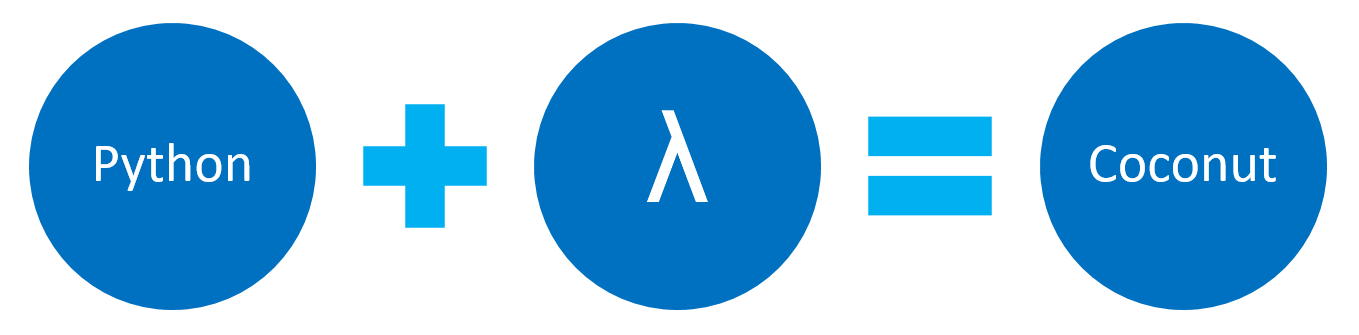
\includegraphics[scale=1.95]{coconut_fp.png}

\large Coconut is a \textbf{variant of Python} built for \textbf{simple, elegant, Pythonic functional programming}.
\end{block}

\begin{block}{Do I Have to Give Up Python?}
\begin{minipage}{0\textwidth}
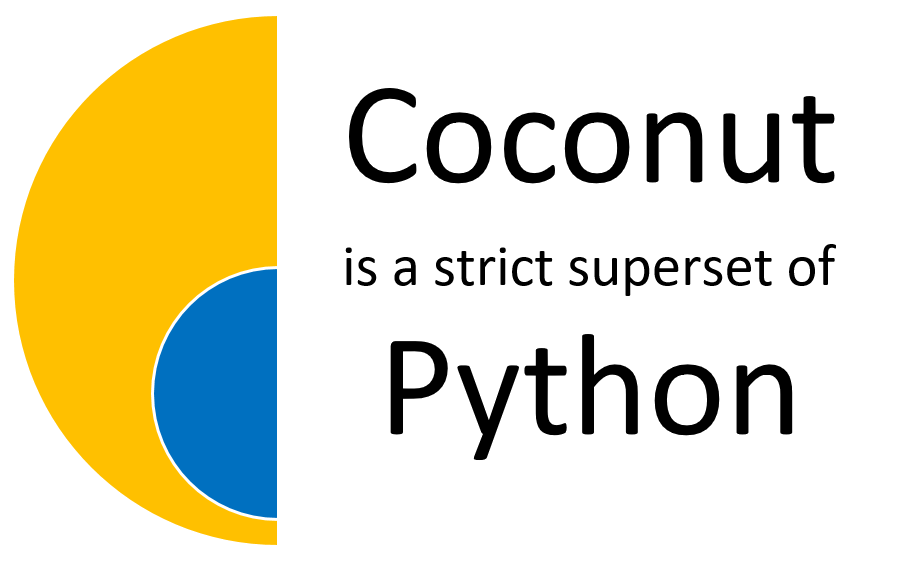
\includegraphics[scale=1.5]{coconut_syntax.png}
\end{minipage} \hfill \begin{minipage}{0.45\textwidth}
\large All valid Python 3 syntax is valid Coconut syntax, which means you can get started writing Coconut just as you would Python.
\end{minipage}
\end{block}

\begin{block}{How Does Coconut Work?}

\includegraphics[scale=2]{coconut_compilation.png}

Coconut compiles to \textbf{any Python version or implementation}, allowing you to write and maintain one code base for any version of Python you want to run your code on.
\end{block}

\begin{block}{Why Use Coconut?}
Coconut adds to Python built-in, syntactical support for:
\begin{columns}
\begin{column}{.5\textwidth}
\begin{itemize}
\item pattern-matching
\item algebraic data types
\item destructuring assignment
\item partial application
\item lazy lists
\item function composition
\end{itemize}
\end{column}
\begin{column}{.5\textwidth}
\begin{itemize}
\item prettier lambdas
\item infix notation
\item pipeline-style programming
\item operator functions
\item tail call optimization
\item parallel programming
\end{itemize}
\end{column}
\end{columns}

\vspace{.01\textheight}

\hspace{.5\textwidth} \ellipsis~ and much more!
\end{block}


\end{column} % End of the first column
\begin{column}{.01\textwidth}\end{column} % Empty spacer column
\begin{column}{.32\textwidth} % The second column

\begin{block}{Coconut Does Pattern-Matching}
\begin{Verbatim}[commandchars=\\\{\}]
\PY{k}{match} \PY{p}{[}\PY{n}{head}\PY{p}{]} \PY{o}{+} \PY{n}{tail} \PY{o+ow}{in} \PY{p}{[}\PY{l+m+mi}{0}\PY{p}{,} \PY{l+m+mi}{1}\PY{p}{,} \PY{l+m+mi}{2}\PY{p}{,} \PY{l+m+mi}{3}\PY{p}{]}\PY{p}{:}
    \PY{n+nb}{print}\PY{p}{(}\PY{n}{head}\PY{p}{,} \PY{n}{tail}\PY{p}{)}

\PY{k}{def} \PY{n+nf}{factorial}\PY{p}{(}\PY{n}{n}\PY{p}{)}\PY{p}{:}
    \PY{l+s+sd}{\PYZdq{}\PYZdq{}\PYZdq{}Compute n! where n is an integer \PYZgt{}= 0.\PYZdq{}\PYZdq{}\PYZdq{}}
    \PY{k}{case} \PY{n}{n}\PY{p}{:}
        \PY{k}{match} \PY{l+m+mi}{0}\PY{p}{:}
            \PY{k}{return} \PY{l+m+mi}{1}
        \PY{k}{match} \PY{n}{\PYZus{}} \PY{o+ow}{is} \PY{n+nb}{int} \PY{k}{if} \PY{n}{n} \PY{o}{\PYZgt{}} \PY{l+m+mi}{0}\PY{p}{:}
            \PY{k}{return} \PY{n}{n} \PY{o}{*} \PY{n}{factorial}\PY{p}{(}\PY{n}{n}\PY{o}{\PYZhy{}}\PY{l+m+mi}{1}\PY{p}{)}


\PY{k}{def} \PY{n+nf}{quick\PYZus{}sort}\PY{p}{(}\PY{p}{[}\PY{p}{]}\PY{p}{)} \PY{o}{=} \PY{p}{[}\PY{p}{]}

\PY{o}{@}\PY{n+nb}{addpattern}\PY{p}{(}\PY{n}{quick\PYZus{}sort}\PY{p}{)}
\PY{k}{def} \PY{n+nf}{quick\PYZus{}sort}\PY{p}{(}\PY{p}{[}\PY{n}{head}\PY{p}{]} \PY{o}{+} \PY{n}{tail}\PY{p}{)} \PY{o}{=}
    \PY{l+s+sd}{\PYZdq{}\PYZdq{}\PYZdq{}Sort a sequence using quick sort.\PYZdq{}\PYZdq{}\PYZdq{}}
    \PY{p}{(}\PY{n}{quick\PYZus{}sort}\PY{p}{(}\PY{p}{[}\PY{n}{x} \PY{k}{for} \PY{n}{x} \PY{o+ow}{in} \PY{n}{tail} \PY{k}{if} \PY{n}{x} \PY{o}{\PYZlt{}} \PY{n}{head}\PY{p}{]}\PY{p}{)}
        \PY{o}{+} \PY{p}{[}\PY{n}{head}\PY{p}{]}
        \PY{o}{+} \PY{n}{quick\PYZus{}sort}\PY{p}{(}\PY{p}{[}\PY{n}{x} \PY{k}{for} \PY{n}{x} \PY{o+ow}{in} \PY{n}{tail} \PY{k}{if} \PY{n}{x} \PY{o}{\PYZgt{}}\PY{o}{=} \PY{n}{head}\PY{p}{]}\PY{p}{)}\PY{p}{)}
\end{Verbatim}
\end{block}

\begin{block}{Coconut Does Algebraic Data Types}
\begin{Verbatim}[commandchars=\\\{\}]
\PY{k}{data} \PY{n+nc}{vector2}\PY{p}{(}\PY{n}{x}\PY{p}{,} \PY{n}{y}\PY{p}{)}\PY{p}{:}
    \PY{l+s+sd}{\PYZdq{}\PYZdq{}\PYZdq{}Immutable two\PYZhy{}element vector.\PYZdq{}\PYZdq{}\PYZdq{}}
    \PY{k}{def} \PY{n+nf}{\PYZus{}\PYZus{}abs\PYZus{}\PYZus{}}\PY{p}{(}\PY{n+nb+bp}{self}\PY{p}{)}\PY{p}{:}
        \PY{k}{return} \PY{p}{(}\PY{n+nb+bp}{self}\PY{o}{.}\PY{n}{x}\PY{o}{*}\PY{o}{*}\PY{l+m+mi}{2} \PY{o}{+} \PY{n+nb+bp}{self}\PY{o}{.}\PY{n}{y}\PY{o}{*}\PY{o}{*}\PY{l+m+mi}{2}\PY{p}{)}\PY{o}{*}\PY{o}{*}\PY{o}{.}\PY{l+m+mi}{5}


\PY{k}{data} \PY{n+nc}{Empty}\PY{p}{(}\PY{p}{)}
\PY{k}{data} \PY{n+nc}{Leaf}\PY{p}{(}\PY{n}{n}\PY{p}{)}
\PY{k}{data} \PY{n+nc}{Node}\PY{p}{(}\PY{n}{l}\PY{p}{,} \PY{n}{r}\PY{p}{)}

\PY{k}{def} \PY{n+nf}{size}\PY{p}{(}\PY{n}{Empty}\PY{p}{(}\PY{p}{)}\PY{p}{)} \PY{o}{=} \PY{l+m+mi}{0}

\PY{o}{@}\PY{n+nb}{addpattern}\PY{p}{(}\PY{n}{size}\PY{p}{)}
\PY{k}{def} \PY{n+nf}{size}\PY{p}{(}\PY{n}{Leaf}\PY{p}{(}\PY{n}{n}\PY{p}{)}\PY{p}{)} \PY{o}{=} \PY{l+m+mi}{1}

\PY{o}{@}\PY{n+nb}{addpattern}\PY{p}{(}\PY{n}{size}\PY{p}{)}
\PY{k}{def} \PY{n+nf}{size}\PY{p}{(}\PY{n}{Node}\PY{p}{(}\PY{n}{l}\PY{p}{,} \PY{n}{r}\PY{p}{)}\PY{p}{)} \PY{o}{=} \PY{n}{size}\PY{p}{(}\PY{n}{l}\PY{p}{)} \PY{o}{+} \PY{n}{size}\PY{p}{(}\PY{n}{r}\PY{p}{)}
\end{Verbatim}
\end{block}


\end{column} % End of the second column
\begin{column}{.01\textwidth}\end{column} % Empty spacer column
\begin{column}{.32\textwidth} % The third column


\begin{block}{Coconut Does Tail Call Optimization}
\begin{Verbatim}[commandchars=\\\{\}]
\PY{k}{def} \PY{n+nf}{factorial}\PY{p}{(}\PY{l+m+mi}{0}\PY{p}{,} \PY{n}{acc}\PY{o}{=}\PY{l+m+mi}{1}\PY{p}{)} \PY{o}{=} \PY{n}{acc}

\PY{o}{@}\PY{n+nb}{addpattern}\PY{p}{(}\PY{n}{factorial}\PY{p}{)}
\PY{k}{def} \PY{n+nf}{factorial}\PY{p}{(}\PY{n}{n} \PY{o+ow}{is} \PY{n+nb}{int}\PY{p}{,} \PY{n}{acc}\PY{o}{=}\PY{l+m+mi}{1} \PY{k}{if} \PY{n}{n} \PY{o}{\PYZgt{}} \PY{l+m+mi}{0}\PY{p}{)} \PY{o}{=}
    \PY{l+s+sd}{\PYZdq{}\PYZdq{}\PYZdq{}Compute n! where n is an integer \PYZgt{}= 0.\PYZdq{}\PYZdq{}\PYZdq{}}
    \PY{n}{factorial}\PY{p}{(}\PY{n}{n}\PY{o}{\PYZhy{}}\PY{l+m+mi}{1}\PY{p}{,} \PY{n}{acc}\PY{o}{*}\PY{n}{n}\PY{p}{)}


\PY{k}{def} \PY{n+nf}{is\PYZus{}even}\PY{p}{(}\PY{l+m+mi}{0}\PY{p}{)} \PY{o}{=} \PY{k+kc}{True}
\PY{o}{@}\PY{n+nb}{addpattern}\PY{p}{(}\PY{n}{is\PYZus{}even}\PY{p}{)}
\PY{k}{def} \PY{n+nf}{is\PYZus{}even}\PY{p}{(}\PY{n}{n} \PY{o+ow}{is} \PY{n+nb}{int} \PY{k}{if} \PY{n}{n} \PY{o}{\PYZgt{}} \PY{l+m+mi}{0}\PY{p}{)} \PY{o}{=} \PY{n}{is\PYZus{}odd}\PY{p}{(}\PY{n}{n}\PY{o}{\PYZhy{}}\PY{l+m+mi}{1}\PY{p}{)}

\PY{k}{def} \PY{n+nf}{is\PYZus{}odd}\PY{p}{(}\PY{l+m+mi}{0}\PY{p}{)} \PY{o}{=} \PY{k+kc}{False}
\PY{o}{@}\PY{n+nb}{addpattern}\PY{p}{(}\PY{n}{is\PYZus{}odd}\PY{p}{)}
\PY{k}{def} \PY{n+nf}{is\PYZus{}odd}\PY{p}{(}\PY{n}{n} \PY{o+ow}{is} \PY{n+nb}{int} \PY{k}{if} \PY{n}{n} \PY{o}{\PYZgt{}} \PY{l+m+mi}{0}\PY{p}{)} \PY{o}{=} \PY{n}{is\PYZus{}even}\PY{p}{(}\PY{n}{n}\PY{o}{\PYZhy{}}\PY{l+m+mi}{1}\PY{p}{)}
\end{Verbatim}
\end{block}

\begin{block}{Coconut Does Much, Much More}
\begin{Verbatim}[commandchars=\\\{\}]
\PY{l+s+s2}{\PYZdq{}}\PY{l+s+s2}{hello, world!}\PY{l+s+s2}{\PYZdq{}} \PY{o}{|\PYZgt{}} \PY{n+nb}{print}

\PY{n}{product} \PY{o}{=} \PY{n+nb}{reduce}\PY{o}{\PYZdl{}}\PY{p}{(}\PY{o}{*}\PY{p}{)}

\PY{k}{def} \PY{n+nf}{a} \PY{o}{`}\PY{n}{mod}\PY{o}{`} \PY{n}{b} \PY{o}{=} \PY{n}{a} \PY{o}{\PYZpc{}} \PY{n}{b}
\PY{p}{(}\PY{n}{x} \PY{o}{`}\PY{n}{mod}\PY{o}{`} \PY{l+m+mi}{2}\PY{p}{)} \PY{o}{`}\PY{n+nb}{print}\PY{o}{`}

\PY{p}{\PYZob{}}\PY{l+s+s2}{\PYZdq{}}\PY{l+s+s2}{list}\PY{l+s+s2}{\PYZdq{}}\PY{p}{:} \PY{p}{[}\PY{l+m+mi}{0}\PY{p}{]} \PY{o}{+} \PY{n}{rest}\PY{p}{\PYZcb{}} \PY{o}{=} \PY{p}{\PYZob{}}\PY{l+s+s2}{\PYZdq{}}\PY{l+s+s2}{list}\PY{l+s+s2}{\PYZdq{}}\PY{p}{:} \PY{p}{[}\PY{l+m+mi}{0}\PY{p}{,} \PY{l+m+mi}{1}\PY{p}{,} \PY{l+m+mi}{2}\PY{p}{,} \PY{l+m+mi}{3}\PY{p}{]}\PY{p}{\PYZcb{}}

\PY{k}{def} \PY{n+nf}{zipwith}\PY{p}{(}\PY{n}{f}\PY{p}{,} \PY{o}{*}\PY{n}{args}\PY{p}{)} \PY{o}{=}
    \PY{n+nb}{zip}\PY{p}{(}\PY{o}{*}\PY{n}{args}\PY{p}{)} \PY{o}{|\PYZgt{}} \PY{n+nb}{map}\PY{o}{\PYZdl{}}\PY{p}{(}\PY{n}{items} \PY{o}{\PYZhy{}\PYZgt{}} \PY{n}{f}\PY{p}{(}\PY{o}{*}\PY{n}{items}\PY{p}{)}\PY{p}{)}

\PY{k}{def} \PY{n+nf}{natural\PYZus{}nums}\PY{p}{(}\PY{n}{n}\PY{o}{=}\PY{l+m+mi}{0}\PY{p}{)} \PY{o}{=}
    \PY{l+s+sd}{\PYZdq{}\PYZdq{}\PYZdq{}Infinite sequence of natural numbers.\PYZdq{}\PYZdq{}\PYZdq{}}
    \PY{p}{(}\PY{n}{n}\PY{p}{,}\PY{p}{)} \PY{o}{::} \PY{n}{natural\PYZus{}nums}\PY{p}{(}\PY{n}{n}\PY{o}{+}\PY{l+m+mi}{1}\PY{p}{)}

\PY{o}{@}\PY{n+nb}{recursive\PYZus{}iterator}
\PY{k}{def} \PY{n+nf}{fib\PYZus{}seq}\PY{p}{(}\PY{p}{)} \PY{o}{=}
    \PY{l+s+sd}{\PYZdq{}\PYZdq{}\PYZdq{}Infinite sequence of fibonacci numbers.\PYZdq{}\PYZdq{}\PYZdq{}}
    \PY{p}{(}\PY{l+m+mi}{1}\PY{p}{,} \PY{l+m+mi}{2}\PY{p}{)} \PY{o}{::} \PY{n+nb}{map}\PY{p}{(}\PY{p}{(}\PY{o}{+}\PY{p}{)}\PY{p}{,} \PY{n}{fib\PYZus{}seq}\PY{p}{(}\PY{p}{)}\PY{p}{,} \PY{n}{fib\PYZus{}seq}\PY{p}{(}\PY{p}{)}\PY{o}{\PYZdl{}}\PY{p}{[}\PY{l+m+mi}{1}\PY{p}{:}\PY{p}{]}\PY{p}{)}

\PY{n}{fib\PYZus{}seq}\PY{p}{(}\PY{p}{)}\PY{o}{\PYZdl{}}\PY{p}{[}\PY{p}{:}\PY{l+m+mi}{100}\PY{p}{]} \PY{o}{|\PYZgt{}} \PY{n+nb}{parallel\PYZus{}map}\PY{o}{\PYZdl{}}\PY{p}{(}\PY{n+nb}{pow}\PY{o}{\PYZdl{}}\PY{p}{(}\PY{k}{?}\PY{p}{,} \PY{l+m+mi}{2}\PY{p}{)}\PY{p}{)} \PY{o}{|\PYZgt{}} \PY{n+nb}{list}
\end{Verbatim}
\end{block}


\end{column} % End of the third column
\begin{column}{.009\textwidth}\end{column} % Empty spacer column

\end{columns} % End of all the columns in the poster
\end{frame} % End of the enclosing frame
\end{document}
